\documentclass[13]{article}
\newtheorem{exer}{Question}
\usepackage[margin=0.5in]{geometry}
\newtheorem{sln}{Solution}
\usepackage{graphicx}
\newtheorem{note}{Note}
\begin{document}
\section{Lecture 1}
\begin{exer}
Material Science vs Materials Engineering ?
\end{exer}
\textbf{Materials Science} involves investigating relationships between structures and properties of materials. While \textbf{Materials Engineering} involves designing/engineering the structure of a material to produce a predetermined set of properties using relations of structure-body. So a material scientist   develops/synthesizes new materials whereas the engineer creates products using those existing materials and/or develop techniques for processing materials.
\begin{exer}
What is the structure of a material.
\end{exer}
\textbf{Structure} in general refers to the arrangement of material's internal components . \\
\textbf{Subatomic Structure} involves electrons within the individual atoms and other particles inside the nuclei.\\
\textbf{Atomic}: Organization of atoms or molecules relative  to one another. \\
\textbf{Microscopic}: Groups of atoms that are normally agglomerated together\\
\textbf{Macroscopic}: seen using the naked eye.
\begin{exer}
What is a Property of a material ?
\end{exer}
It's a material's trait in terms of the kind and magnitude of a response to a specific imposed stimulus. 
\begin{exer}
What are Mechanical Properties of a material ?
\end{exer}
It's the response or deformation of a material due to an applied load or force.
\begin{exer}
Mechanical Properties Standards ?
\end{exer}
Mechanical properties are measured using standardized testing
techniques coordinated by professional societies such as the ASTM American Society for Testing and Materials. 
\begin{exer}
Processing and Performance?
\end{exer}
\textbf{Processing} refers to the methodology or techniques by which a material is prepared. \\
\textbf{Performance} indicates how good the materials will do its function.
\begin{exer}
Processing and Performance and so on relations.
\end{exer}
The \textbf{structure}  of a material depends on how it is \textbf{processed} , and material's \textbf{performance} is a function of its \textbf{properties} . And the properties is affected by the structure. 
\begin{exer}
Classification of Materials
\end{exer}
C-MPC
\begin{itemize}

\item Metals
\begin{itemize}

	\item Dense atomic packing (Metallic bonding)
	\item Non localized electrons (good conductors)
	\item Metals are dense because they are made of heavy atoms, packed 
densely together (iron, for instance, has an atomic weight of 56).
\end{itemize}
\item Ceramics
\begin{itemize}

\item Compounds of metallic and non metallic elements
\item Brittle
\item Ceramics, for the most part, have lower densities than metals because
	they contain light nonmetals like O, N or C atoms.
\end{itemize}
\item Polymers
	\begin{itemize}
	
	\item Most are organic compounds based on C and H
	\item Low Density, and Ductile.
	\item Polymers have low densities because they are largely made of
		light carbon (atomic weight: 12) and hydrogen (atomic weight:
		1) 	
	\end{itemize}
\item Composites
\begin{itemize}

\item Physical binding between materials from other classes to get intermediate properties.

\end{itemize}
\end{itemize}
\begin{exer}
What does Failure mean ?
\end{exer}
The end goal of studying property structure and processing relationships is that a product or component can perform its function and not fail in service. \\ Failure does not necessarily mean fracture. Failure to perform a function can be due to
\begin{itemize}

	\item \textbf{Excessive Elastic deformation:}  excessive deflection of closely mating
	parts can result  in interference and damage to the parts, this type
	of failure is controlled by the modulus of elasticity, not by the
	strength of the material. Generally, little metallurgical control can
	be exercised over the  elastic modulus. The most effective way to
	increase the stiffness  of a member is usually by changing its shape
	and increasing the dimensions of its cross section.
\item \textbf{Yielding and excessive plastic deformation:}  occurs when the elastic
	limit of the metal has been  exceeded. Yielding produces permanent
	change of shape, which may prevent the part from 
\item \textbf{Fracture:}  The formation of a crack which can result in complete
	disruption of continuity of the member  constitutes fracture. A part
	made from a ductile metal which is loaded statically rarely
	fractures because it will first fail by excessive plastic
	deformation.  Fracture could be a combined effect of stress and other
	factors such as corrosion for example.


\end{itemize}
\section{Lecture 2}
\begin{exer}
Types of bonding ?
\end{exer}
\begin{itemize}

	\item \textbf{Ionic:}  Compounds that consist of Metallic + non-metallic elements.
	Atoms of a metallic element easily give up their valence electrons to
	the nonmetallic atoms. In the process all the atoms acquire stable or
	inert gas configurations and, in addition, an electrical charge; that
	is, they become ions. identical to that of argon. In sodium chloride,
	all the sodium and chlorine exist as ions.  The attractive bonding
	forces are coulombic; that is, positive and negative ions attract
	each other.
\item \textbf{Covalent}: In covalent bonding stable electron configurations are assumed by \textbf{the sharing}  of electrons between adjacent atoms.
\item \textbf{Metallic}: is found in metals and their alloys. With this
	model, these valence electrons are not bound to any particular atom
	in the solid and are more or less free to drift throughout the entire
	metal.  They may be thought of as belonging to the metal as a whole,
	or forming a \textbf{‘‘sea of electrons’’}  or an \textbf{‘‘electron
	cloud.’’}. The remaining nonvalence electrons and atomic nuclei form
	what are called ion cores, which possess a net positive charge  equal
	in magnitude to the total valence  
\end{itemize} 
\begin{exer}
What are types of Crystal Structures?
\end{exer}
\begin{itemize}

	\item \textbf{Single Crystalline}: Atoms are arranged in regular repetitive manner having long range order (long range periodic structure) 
	\item \textbf{Polycrystalline}: Many individual crystals (local
		periodicity)
	\item\textbf{ Amorphous}: Atomic arrangement does not have any order

\end{itemize}
\begin{exer}
How to describe a crystal structure ?
\end{exer}
Using a lattice and a motif;
\begin{itemize}

	\item \textbf{lattice}: Description of the pattern of motifs/basis. (The whole pattern)
	\item \textbf{motif}: the basis that is being repeated. (an atom or a group of atoms)

\end{itemize}
\begin{exer}
What is a Bravais Lattice ?
\end{exer}
It is an infinite arrangement of points or atoms in space that has the following property: The lattice looks exactly the same when viewed from any lattice point.
\begin{exer}
How to represent a space lattice ?
\end{exer}
using three translational vectors and three angles between each pair of these lattice vectors \textbf{(Lattice parameters).
} \begin{exer}
How is a unit cell defined ?
\end{exer}
Using these vectors and angels we represent the smallest unit of the crystal structure that is when repeated along the three translational axes will produce the crystal structure.
\begin{exer}
How many Bravais lattices there exist ?
\end{exer}
14. There are only 14 unique [patterns that are mathematically proven to fill a 3D space that possess translational symmetry.
\begin{exer}
How many crystal systems there exist ?
\end{exer}
7 and are Cubic, Hexagonal, Tetragonal, Rhombohedral, Orthohomobic, Monoclinic and Triclinic.
\begin{exer}
Define the Correspondence principle.
\end{exer}
Usually the external shape of a material is influenced by the internal structure (crystal system). Snow flakes is a good example of this principle.
\begin{exer}
What are our unit cells of interest in this course ?
\end{exer}
The seven crustal systems give up 14 different unit cells, we will focus on only four of them; \\
SC - BCC - FCC - HCP.
\begin{exer}
What is the coordination number in a unit cell?
\end{exer}
The number of each atom's nearest neighbours.
\begin{exer}
What is the atomic packing factor in a unit cell APF?
\end{exer}
represents the total volume of the unit cell that is occupied by atoms. APF of 0.7 means the unit cell is 70\% fill with atoms.
\begin{exer}
Number of atoms per unit cell in Simple Cubic unit cell?
\end{exer}

\[
N = 8 corners * \frac{1}{8} = 1 atom 
.\]
\begin{center}
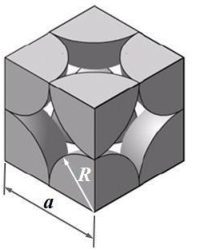
\includegraphics[scale=0.5]{figures/6.png} 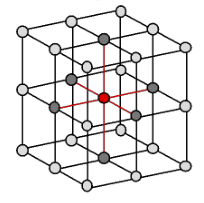
\includegraphics[scale=0.5]{figures/7.png}
\end{center}
\begin{exer}
Examples of Simple cubic?
\end{exer}
Polonium (PO)
\begin{exer}
What is the relationship between r and a in Simple Cubic unit cell?
\end{exer}
a = 2R.
\begin{exer}
Coordination number in Simple Cubic unit cell?
\end{exer}
\[
CN=6
.\] 
\begin{exer}
The atomic packing factor in Simple Cubic unit cell?
\end{exer}
\[
	APF = \frac{volume of atoms}{volume of unit cell} = \frac{1* \frac{4}{3} * \pi R^3}{a^3}= \frac{1* \frac{4}{3} * \pi R^3}{(2R)^3} = 0.523
.\] 
52\% of it is filled with atoms. 
\begin{exer}
Number of atoms per unit cell in Body Centred Cube unit cell?
\end{exer}
\[
N = 8 corners * \frac{1}{8} + 1 centered = 2 atom 
.\]
\begin{center}
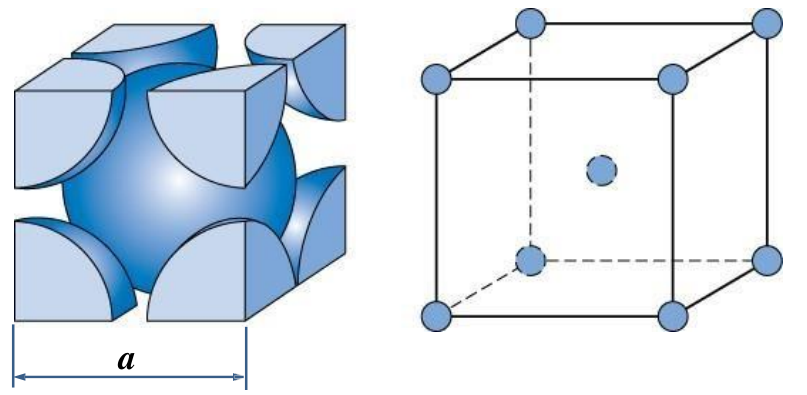
\includegraphics[scale=0.5]{figures/8.png} 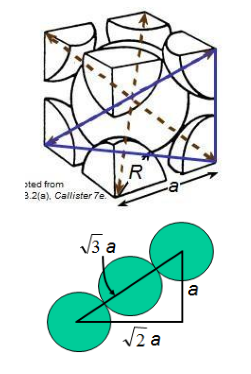
\includegraphics[scale=0.5]{figures/9.png}
\end{center}

\begin{exer}
Examples of BCC ?
\end{exer}
alpha-iron (a-Fe), Tungsten (W), Chromium (Cr), Tantalum (Ta), Molybdenum (Mo)
\begin{exer}
What is the relationship between r and a in Body Centred Cube unit cell?
\end{exer}
$a = \frac{4R}{\sqrt{3}}$
\begin{exer}
Coordination number in Body Centred Cube unit cell?
\end{exer}
\[
CN=8
.\] 
\begin{exer}
The atomic packing factor in Body Centred Cube unit cell?
\end{exer}
\[
	APF = \frac{volume of atoms}{volume of unit cell} = \frac{2* \frac{4}{3} * \pi R^3}{a^3}= \frac{1* \frac{4}{3} * \pi R^3}{(4R/\sqrt{3})^3}= 0.68
.\] 
68 \% of it is filled with atoms. 
\begin{exer} Number of atoms per unit cell in Face Centred Cubic (FCC) unit cell?
\end{exer}
\begin{exer}
Examples of FCC?
\end{exer}
Gamma iron (y-Fe), aluminium (Al), Gold(Au), Nickel (Ni), Silver (Ag), Copper (Cu), Platinum (Pt), Lead (Pb). 
\[
N = 8 corners * \frac{1}{8} + 6* \frac{1}{2}  = 4 atom 
.\]

\begin{center}
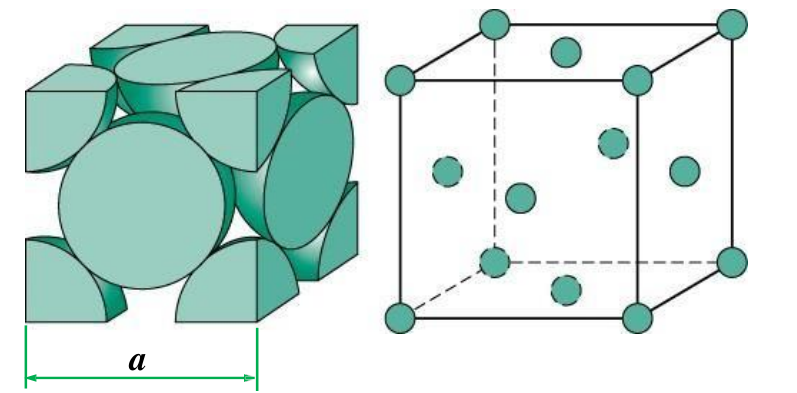
\includegraphics[scale=0.5]{figures/10.png} 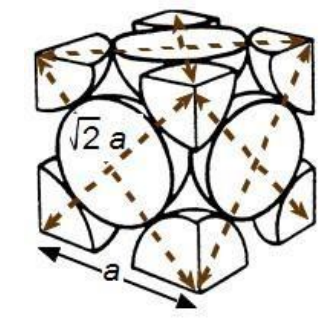
\includegraphics[scale=0.5]{figures/11.png}
\end{center}
\begin{exer}
What is the relationship between r and a in Face Centred Cubic (FCC) unit cell?
\end{exer}
\[
	a = \frac{4R}{\sqrt{2}} 
.\] 
\begin{exer}
Coordination number in Face Centred Cubic (FCC) unit cell?
\end{exer}
\[
CN=12
.\] 
\begin{exer}
The atomic packing factor in Face Centred Cubic (FCC) unit cell?
\end{exer}
\[
	APF = \frac{volume of atoms}{volume of unit cell} = \frac{4* \frac{4}{3} * \pi R^3}{a^3}= \frac{4* \frac{4}{3} * \pi R^3}{(4R/\sqrt{2})^3} = 0.74
.\] 
74\% of it is filled with atoms. 
\begin{exer}
Number of atoms per unit cell in  Hexagonal Close Packed (HCP) unit cell?
\end{exer}
\[
N = 12* \frac{1}{6}  + 2 * \frac{1}{2} + 3 = 6 atoms
.\]
\begin{center}
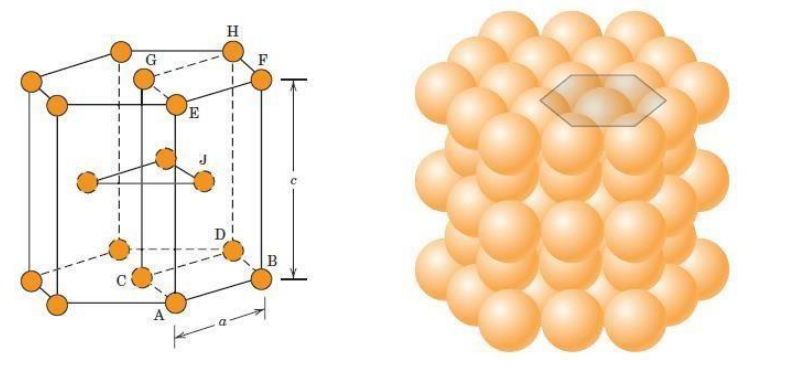
\includegraphics[scale=0.5]{figures/12.png} 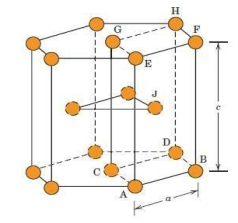
\includegraphics[scale=0.5]{figures/13.png}
\end{center}

\begin{exer}
Examples of HCP ?
\end{exer}
Magnesium (Mg), Zinc (Zn), Cadmium (Cd), Titanium (Ti).
\begin{exer}
What is the relationship between r and a in  Hexagonal Close Packed (HCP) unit cell?
\end{exer}
a = 2R.
\begin{exer}
Coordination number in  Hexagonal Close Packed (HCP) unit cell?
\end{exer}
\[
CN=12
.\] 
\begin{exer}
The atomic packing factor in  Hexagonal Close Packed (HCP) unit cell?
\end{exer}
\[
	APF = \frac{volume of atoms}{volume of unit cell} = \frac{6* \frac{4}{3} * \pi R^3}{0.5*c*a^2*sin(60)}= \frac{6* \frac{4}{3} * \pi R^3}{ \frac{\sqrt{3}}{4} * \sqrt{ \frac{8}{3}}*(2R)^3  } = 0.74
.\] 
74\% of it is filled with atoms. 
\\ c is the height and a is the side length
\begin{exer}
What is theoretical density ?
\end{exer}
Density of a unit cell. 
\[
	\rho = \frac{\textbf{mass of unit cell}}{ \textbf{volume of unit cell} }  
.\]
\[
\rho = \frac{nA}{N_AV_C} 
.\] 
Where: n: number of atoms in a unit cell. \\
A: molecular weight.mass of one mole of a substance in gm/mole \\
Na : Avogadro's  no. =  $6.023*10^{23}$\\
Vc: volume of unit cell. 
\section{Lecture 3}
\begin{exer}
What is \textbf{Polymorphism/Allotropy}? 
\end{exer}
Two or more distinct crystal structures for the same material. 
\begin{exer}
Examples of Polymorphism?
\end{exer}
Carbon can be Graphite, Diamond and Graphene.
\begin{exer}
Define Grain Boundaries ?
\end{exer}
The zone of crystalline mismatch between adjacent grains. The lattice has different orientation on either side of the grain boundary. 
\begin{exer}
	Compare single crystal (GRAIN) and polycrystalline materials in terms of properties.
\end{exer}
\begin{itemize}

\item Single 
	\begin{itemize}
	
	\item Properties vary with direction:\textbf{ anisotropic.
		} 
	\item such as the modulus of elasticity(E) in BCC iron.
	\end{itemize}
\item Poly crystal
\begin{itemize}

\item may or may not vary with direction.
\item if the grains are randomly oriented then it is \textbf{isotopic} .

\end{itemize}
\end{itemize}
\begin{exer}
What is the relationship between grain size and strength of materials ?
\end{exer}
the \textbf{Hall-Petch}  Relationship: When the grain size decreases the strength of the material increases . Inverse Relation.
\begin{exer}
How to measure the Grain Size ?
\end{exer}
The Linear Intercept method where \[
d_x = \frac{L*z}{V*n_x} 
.\]
Where L: length of each line (The longer the better) \\
z: number of lines \\
V: magnification \\
n: number of intercepts.
\begin{exer}
What are Miller Indices/Planes ?
\end{exer}
The reciprocals of the fractional intercepts with the crystallographic axes. Indices are represented in (hkl) parentheses
\begin{exer}
How to calculate Millers ?
\end{exer}
Identify the plane intercepts, take the reciprocal, reduce any fraction by multiplication.\\ 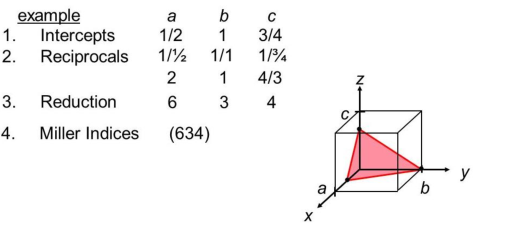
\includegraphics[scale=0.5]{figures/2021-05-16_03-22.png} \\ Note that not all planes are that easy, some planes need you to change the origin, you can avoid this origin changing thing by getting the equation of the plane itself using simple math.
\begin{exer}
What are structure directions ?
\end{exer}
it's simply the direction :) (end point - start point). [uvw]
\begin{exer}
	How to find directions ?
\end{exer}
Get the vector direction (end-start), remove any fraction by multiplication, put the result in square brackets and convert any negative to a bar.
\begin{exer}
	When is a Direction [uvw] is normal to a Plan (hkl) ?
\end{exer}
When u=h, v=k, and w=l in a cubic system.
\begin{exer}
Linear Density?
\end{exer}
The number of atoms per unit length whose centres lie on the direction vector for a specific crystallographic direction. = no.of atoms centred on the direction vector/length of the vector 
\begin{exer}
Planar Density ?
\end{exer}
number of atoms per unit area that are centred on particular crystallographic plane. = no. of atoms centred on a plane/area of the plane.
\begin{exer}
Why are Miller Indices important ?
\end{exer}
Those planes and directions influence;
\begin{itemize}

\item Optical Properties
\item Chemical Reactivity 
\item Surface Tension 
\end{itemize}
\begin{exer}
What do defects affect ?
\end{exer}
Defects are the reason why materials show lower strength than they could.
\begin{exer}
What are types of defects or imperfections in a crystal structure ?
\end{exer}
\begin{itemize}

	\item \textbf{Point defect:}  such as 
	\begin{itemize}
	
		\item\textbf{ Vacancy:}  vacant lattice site, one that is normally occupied but now missing.
		\item \textbf{self-interstitial:}  a one that is crowded. Opposite of a vacancy.
		\item \textbf{small substitional atoms:}  one that is smaller than normal
		\item \textbf{large substitional atoms:}  of course you know.
	\end{itemize}
\item \textbf{Linear defects:}  \begin{itemize}

	\item \textbf{Edge dislocation} : an extra plane of atoms present in the lattice. The atoms above the dislocation lone are squeezed together while those below are pulled apart. (Compression and Tension). The magnitude and direction of the lattice distortion is represented by a \textbf{Burgers Vector} (b). And this dislocation have some strain fields (vector field) that arises at their cores. And of course the strain drops rapidly with distance from the dislocation core.\\
		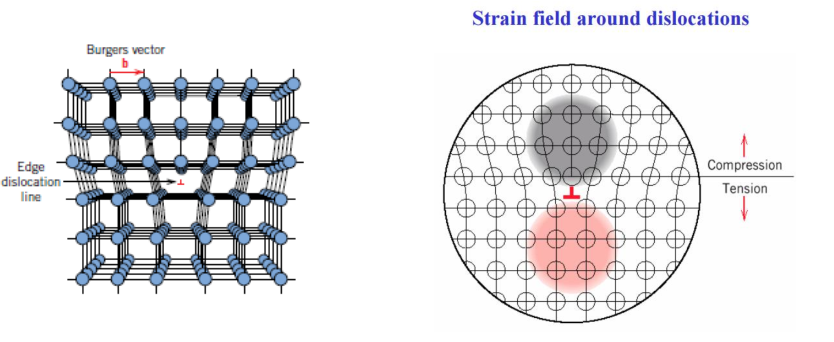
\includegraphics[scale=0.5]{figures/2.png}
	\item \textbf{Screw dislocations. } 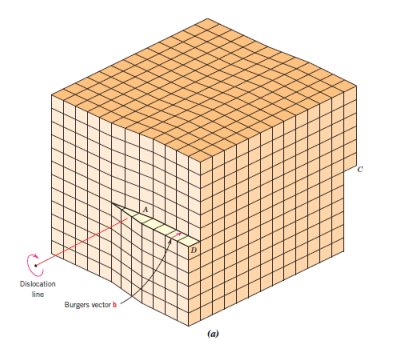
\includegraphics[scale=0.5]{figures/3.png} 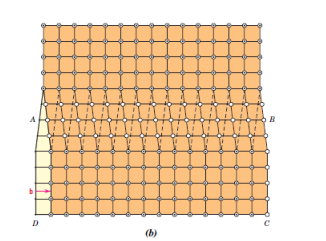
\includegraphics[scale=0.5]{figures/4.png}
\end{itemize}
\item \textbf{Planar defect}: Interfacial defects are boundaries that have
	two dimensions and normally separate regions of the materials that
	have different crystal structures and/or crystallographic
	orientations.  Grain Boundaries are a result of that defect. Various degrees of crystallographic misalignment between adjacent grains are possible.
\\
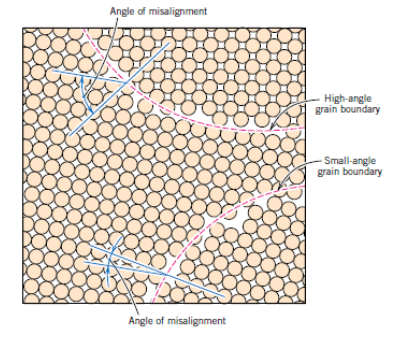
\includegraphics[scale=0.5]{figures/5.png}
\end{itemize}
\end{document}
